\section{Аналитический обзор существующих решений}
\label{sec:alternatives:intro}

Существует целый ряд готовых средств для того, чтобы взаимодействовать с клиентом на сайте и получать о нем как можно более точный профиль данных, например различные CRM системы, Google Analytics и многое другое. У всех есть свои особенности и уникальные возможности, поэтому зачастую используются сразу несколько специализированных средств. 


\subsection{Google Analytics}
\label{sub:alternatives:ga}
Самым популярным средством для сбора статистики данных о пользователе в данный момент является Google Analytics(рисунок~\ref{fig:ga}), которая включает в себя обширные возможности ~\cite{ga}.

\begin{figure}[ht]
\centering
  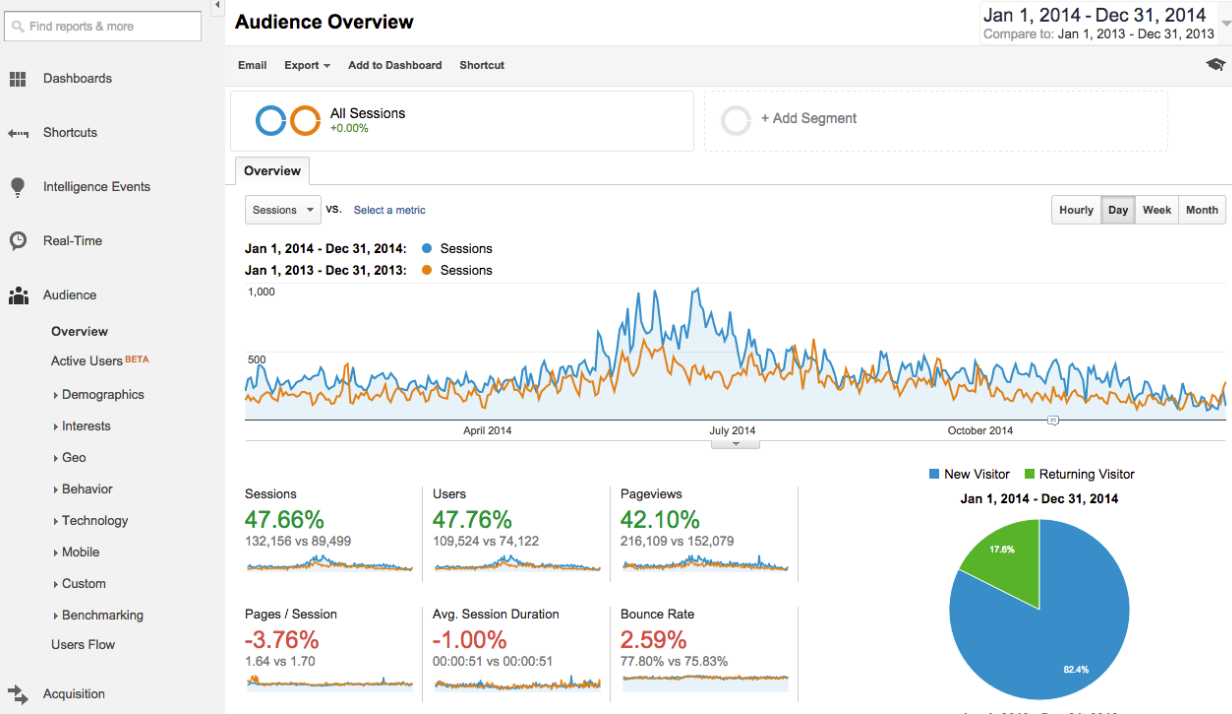
\includegraphics[scale=0.8]{ga.png}  
  \caption{Google Analitics}
	\label{fig:ga}
\end{figure}


Преимущества:
\begin{itemize}
\item способность отслеживать статистику переходов на сайт;
\item способность классифицировать посетителей, что позволяет разрабатывать новые страницы сайта более эффективно с учетом потребностей целевой аудитории;
\item способность отслеживать исходящие ссылки, используемые при продвижении сайта, также необходимые для дальнейшей раскрутки сайта;
\item способность отслеживать ссылки, которые скачивают больше всего;
\item способность отслеживать адреса электронной почты по кликам;
\item практически все коммерческие транзакции прослеживаются при помощи Google Analytics;
\item можно отключить статистику посещений тех, кто обслуживает сайт;
\item Сравнение статистики посещения сайта за разные периоды. Данная возможность идеальна для выявления эффективности работы новых страниц.
\end{itemize}


Недосатки:
\begin{itemize}
\item невозможно отследить трафик, если у пользователя отключены cookies;
\item Google Analytics не может повторно обработать данные, если потерян профиль с настроенными фильтрами;
\item настройка отчетов имеет ограниченное количество параметров;
\item количество отслеживаемых целей также ограничено (настоящее время Google Analytics отслеживает до четырех целей).
\end{itemize}

\subsection{CRM системы}
\label{sub:alternatives:crm}
Раньше CRM системы были доступны только для корпоративного сектора. Исключительно компании с развитой технологической инфраструктурой, огромным штатом сотрудников и достаточным бюджетом могли приобрести CRM систему для автоматизации работы отделов продаж, маркетинга и сервисного обслуживания клиентов.
Постепенно с тем, как увеличивалась скорость Интернет-подключения, появлялись облачные технологии и приобретали свою популярность SaaS решения (англ. software as a service — программное обеспечение как услуга), приобретение CRM систем становилось доступной опцией для любой компании.

Сегодня рынок CRM является динамичным и быстрорастущим. Облачные технологии позволяют легко внедрять CRM системы с нуля, без особых технических хлопот с развертыванием и по низкой стоимости. Далее приведены основные характеристики CRM систем, покупательские критерии, а также сравнения CRM решений от разных поставщиков. Конечно есть свои нюансы, и бизнесы должны полагаться на свои собственные требования при выборе оптимальной CRM системы. Далее рассмотрены базовые параметры, на которые следует обратить внимание при выборе CRM системы:
\begin{itemize}
\item варианты хостинга;
\item наличие мобильного клиента;
\item стоимость;
\item функционал для продаж;
\item функционал для маркетинга;
\item наличие сервисного модуля;
\item возможности хранения документов на дисковых пространствах CRM системы;
\item модуль отчетности.
\end{itemize}

Далее приведен обзор следующих CRM систем: SugarCRM, Salesforce.com, Microsoft Dynamics CRM и Zoho ~\cite{crms}.


\subsubsection{SugarCRM }
\label{sub:alternatives:crm:sugar}
SugarCRM (рисунок~\ref{fig:sugar}) предлагает систему для поддержки процессов продаж, маркетинга и сервисного обслуживания. Стоимость лицензии начинается от \$35 за пользователя в месяц в рамках редакции Professional с возможностью развертывания решения на серверах предприятия и до \$150 за пользователя в месяц за редакцию Ultimate. В рамках подписки на все редакции предоставляется мобильный клиент, а размеры хранилища документов варьируются от 15 Гб в редакции Professional до 250 ГБ – в Ultimate ~\cite{sugar}.

\begin{figure}[h]
\centering
  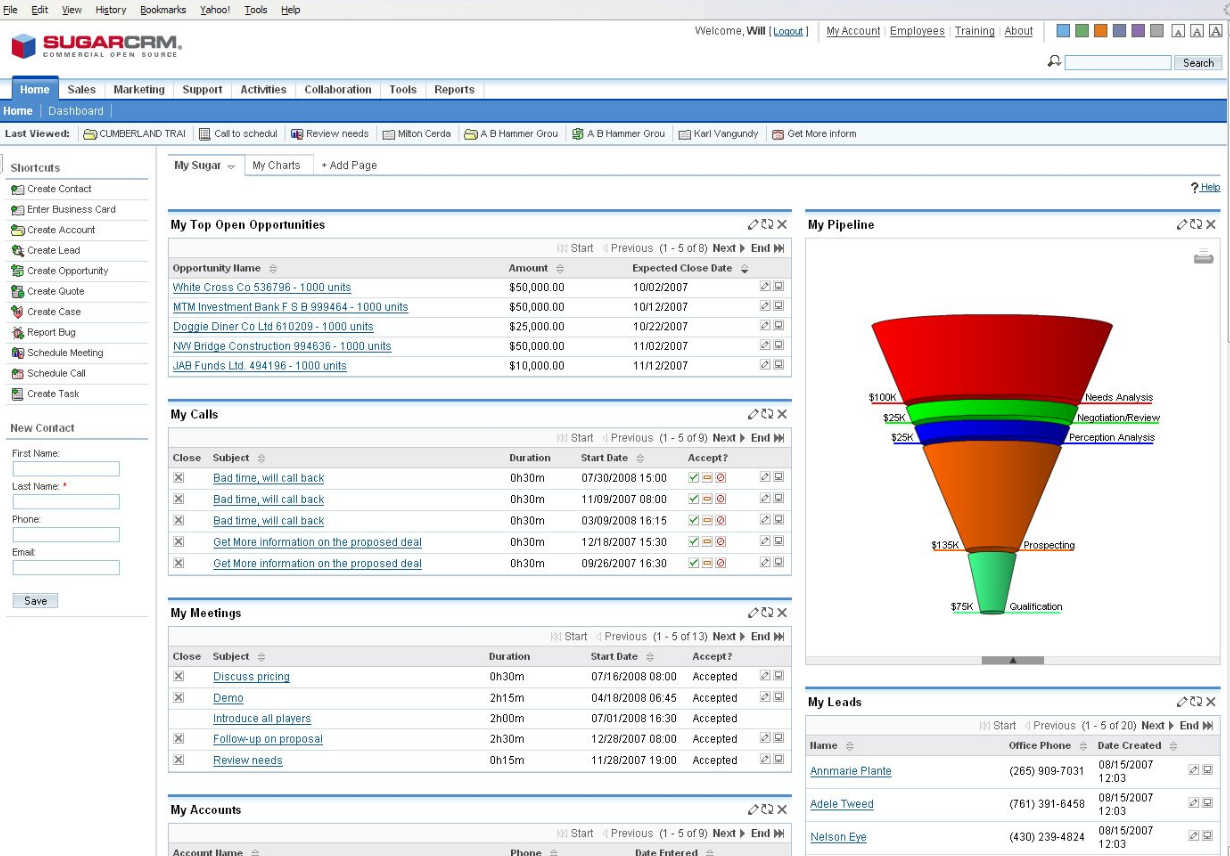
\includegraphics[scale=0.7]{sugarCRM.png}  
  \caption{SugarCRM}
  \label{fig:sugar}
\end{figure}

Основные функциональные возможности SugarCRM:
\begin{itemize}
\item Workflow или автоматические процессы. Позволяет автоматически настраивать события и следить за их выполнением. В продажах этот механизм особенно важен: позволяет создавать новые продажи с различным бюджетом, контролировать пребывание продажи на конкретной стадии и многое другое.
\item Интеграция с SMS. Как и интеграция с социальными сетями стала неотъемлемой частью работы компании, SMS сервисы стали важными каналами коммуникации с клиентами и предоставления сервиса последним. Возможность интегрировать CRM систему и сервис SMS сообщений является важным преимуществом.
\item Функция Web-to-lead. CRM система Sugar также позволяет собирать клиентские данные с веб-сайта компании и автоматически аккумулировать эти данные в CRM системе.
\end{itemize}

Преимущества: 
\begin{itemize}
\item SugarCRM имеет открытый исходный код, поэтому система достаточно гибкая и масштабируемая с возможностью расширения под потребности бизнеса;
\item систему можно достаточно легко настраивать под предпочтения бизнес пользователей.
\end{itemize}

Недостатки: 
\begin{itemize}
\item чтобы пользоваться SugarCRM нужны определенные знания и компетенции, на обучение требуется время.
\end{itemize}



\subsubsection{Salesforce CRM }
\label{sub:alternatives:crm:sf}
Salesforce CRM (рисунок~\ref{fig:sf}) лидирует в сегменте облачных CRM систем уже на протяжении многих лет. Salesforce.com предлагает CRM систему Sales Cloud, которая поставляется в пяти редакциях, начиная с базовой редакции Contact Manager стоимость лицензии которой начинается от \$5 за пользователя в месяц. Наиболее популярная редакция, которая наилучшим образом удовлетворяет бизнес потребности большинства компаний является Enterprise. Ее стоимость составляет \$125 за пользователя в месяц; редакция поставляется с функционалом по ведению и управлению продажами, управлению процессами lead менеджмента, настраиваемыми рабочими столами (dashboard), workflow и возможностями интеграции через API. 

Основные функциональные возможности Salesforce.com:
\begin{itemize}
\item Синхронизация с Outlook. Данные из CRM системы Salesforce автоматически синхронизируются с Outlook, включая контакты, календарь и многое другое.
\item Настраиваемые процессы продаж. Можно адаптировать процессы продаж под модель организации компании. Это играет ключевую роль при выборе CRM системы, потому что продавцам очень важно использовать технологию, в которой доступны не только стандартные процессы.
\item Функция Web-to-lead. Эта функция позволяет компаниям собирать информацию со своих сайтов и генерировать ее внутри CRM системы Salesforce, на основе этих данных создавать лиды.
\item Мобильный доступ в режиме offline. Очень важная опция для полевых продавцов, которые могут вводить данные в CRM систему с мобильного в автономном режиме и позже синхронизировать эти данные в CRM при возобновлении подключения к Интернет.
\item Интеграция через web-сервисы API. Эта опция позволяет CRM системе Salesforce синхронизироваться с другими backend офисными системами, такими как ERP, системами финансового учета, а также дает возможность компаниям расширять функциональность и интегрировать систему с другими технологиями.
\end{itemize}


\begin{figure}[h]
\centering
  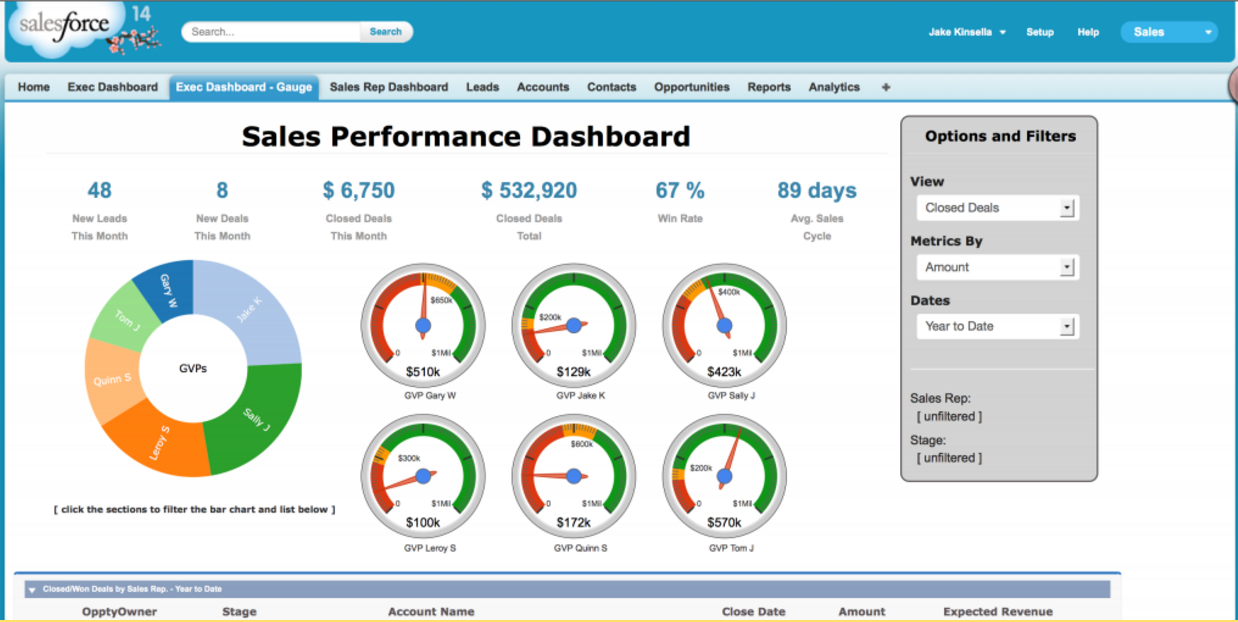
\includegraphics[scale=0.7]{sf.png}  
  \caption{Salesforce CRM}
	\label{fig:sf}
\end{figure}

Преимущества: 
\begin{itemize}
\item гибкость системы, наличие ключевых CRM функций, в том числе визуализация воронки продаж в режиме реального времени;
\item мобильный клиент для всех редакций системы;
\item возможная интеграция с инструментами работы с данными от третьих производителей, такими как Data.com, Twitter, LinkedIn, YouTube и Klout, увеличит производительность работы на всех этапах цикла продажи, от потенциального клиента до клиента.
\end{itemize}

Недостатки: 
\begin{itemize}
\item только облачный вариант развертывания, что ставит под вопрос безопасность клиентских данных для некоторых компаний;
\item стоимость редакций Professional и Enterprise дороже, чем у большинства других игроков рынка.
\end{itemize}


\subsubsection{Microsoft Dynamics CRM }
\label{sub:alternatives:crm:msDM}
Microsoft Dynamics CRM (рисунок~\ref{fig:msDM}) поздно появилась на рынке CRM, и ранние редакции Microsoft CRM не имели большого спроса среди пользователей.  Стоимость этой редакции начинается от \$65 за пользователя в месяц. Dynamics CRM – это технология с полным набором различных функций -- от управления лидами и до заключения продажи, поэтому с помощью Dynamics CRM можно выстраивать полноценные отношения с клиентами. CRM система интегрируется с другими инструментами от Microsoft – программным пакетом Office и Office 365 -- для ведения email коммуникаций, анализа данных и управления документами – однако это все за дополнительную плату ~\cite{msdyn}.


% \FloatBarrier
\begin{figure}[h]
\centering
  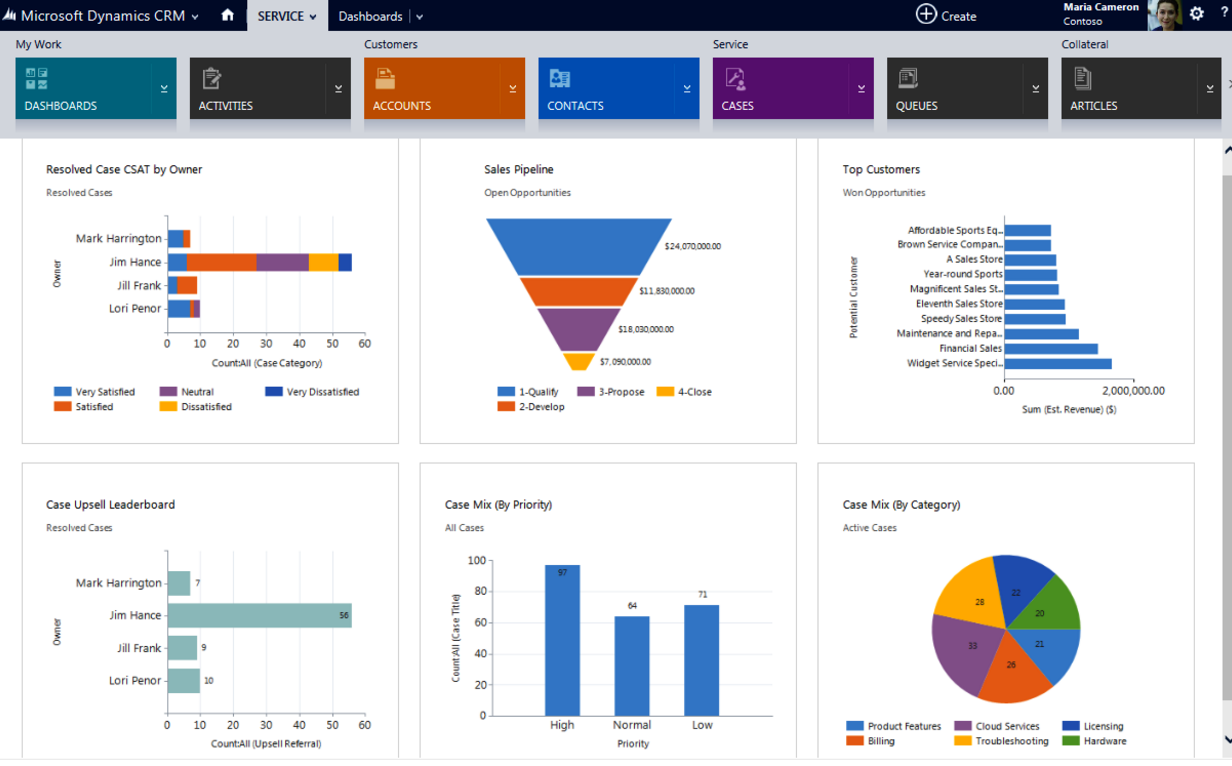
\includegraphics[scale=0.7]{microsoftDM.png}  
  \caption{Microsoft Dynamics CRM}
  \label{fig:msDM}
\end{figure}

Основные функциональные возможности Dynamics CRM:
\begin{itemize}
\item интеграция с Microsoft Office;
\item Настраиваемые отчеты и рабочие столы. Есть возможность генерировать кастомизированные отчеты для руководства.
\item Механизм workflow для настройки бизнес процессов. Можно планировать и оптимизировать бизнес-процессы в CRM системе Dynamics с помощью данного инструмента.
\item Интеграция через web-сервисы. Microsoft синхронизируется с другими backend офисными системами, такими как ERP системы, системы финансового учета и др.
\item Мобильный доступ. Microsoft разработала систему Dynamics с доступной мобильной версией.
\item Настраиваемые сущности. Эта функция позволяет третьим производителям дорабатывать функционал готовой CRM системы. Например, настроенная сущность <<Проект>> может быть создана для управления отношениями между контактами и контрагентами с поддержкой функционала существующих сущностей системы.
\item Соглашение о качестве предоставляемых услуг. Microsoft подписывает соглашение о качестве предоставляемых услуг, которое обеспечивает компаниям безопасность клиентских данных, а также страхует их от потери данных и других потенциальных угроз.
\end{itemize}

Преимущества: 
\begin{itemize}
\item Microsoft обладает богатым функционалом для увеличения лидов до продажи или сервисного обращения;
\item Microsoft хорошо интегрируется с другими продуктами для повышения производительности бизнеса, такими как Office и Office 365.
\end{itemize}

Недостатки: 
\begin{itemize}
\item решение Microsoft CRM стоит очень дорого;
\item известно больше как преемник тенденций, а не новатор.
\end{itemize}


\subsubsection{Zoho CRM }
\label{sub:alternatives:crm:zoho}
Zoho CRM (рисунок~\ref{fig:zoho}) предлагает различные онлайн продукты и облачные технологии; CRM система – одна из них. Стоимость владения системой довольно низкая; система поставляется на бесплатной основе, если количество пользователей не превышает 3 единицы, и может послужить хорошей отправной точкой для представителей малого бизнеса. На таких условиях предоставляется базовый функционал управления лидами, продажами, контрагентами и контактами ~\cite{zoho}. 

\pagebreak
\begin{figure}[h]
\centering
  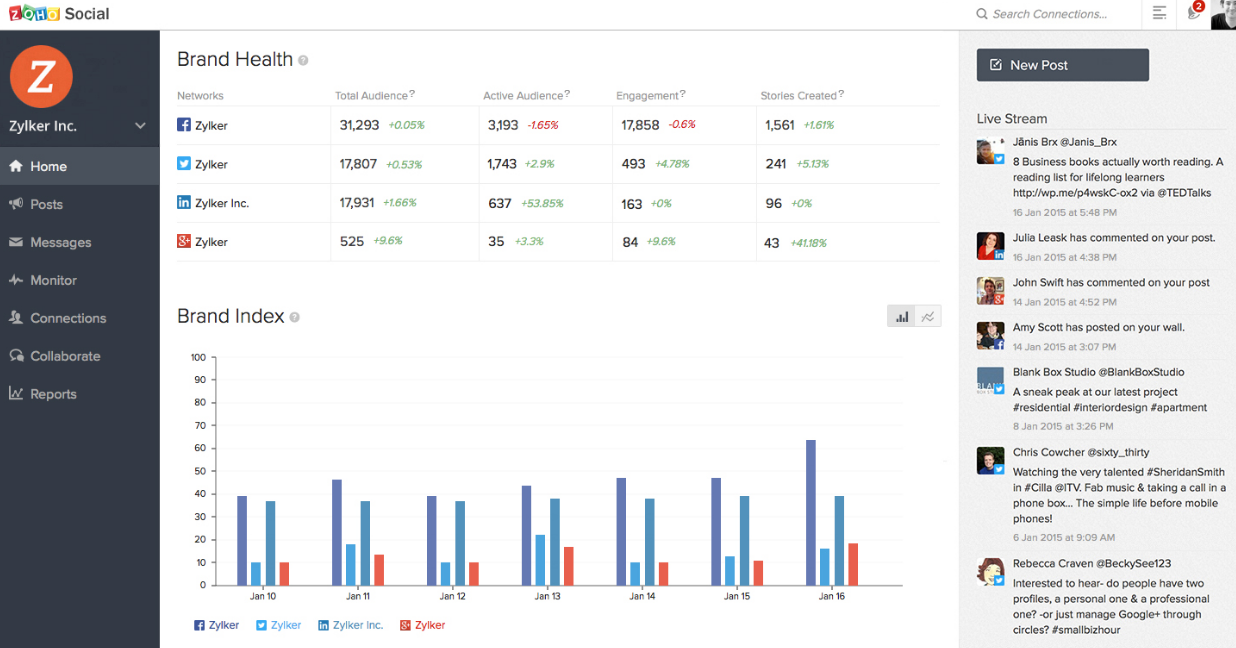
\includegraphics[scale=0.7]{zoho.png}  
  \caption{Zoho CRM}
  \label{fig:zoho}
\end{figure}

Основные функциональные возможности Zoho:
\begin{itemize}
\item Функция Web to lead, case формы. Пользователи могут собирать данные из форм непосредственно в CRM систему Zoho.
\item Настраиваемые рабочие столы. На рабочий стол пользователи могут выводить нужную им информацию для оперативной работы.
\item Автоматизация маркетинга. Инструмент автоматизации маркетинга автоматически сегментирует целевую аудиторию компании для точечного обращения и позволяет измерять затраченные усилия.
\item Интеграция с Twitter и Facebook. Увеличение роли социальных сетей в улучшении клиентского опыта. Необходимость отслеживать поведения клиентов в социальных медиа, а также потребность в повышении эффективности маркетинга, делают интеграцию с социальными платформами обязательным элементом для CRM систем.
\end{itemize}

Преимущества: 
\begin{itemize}
\item сбор данные веб-форм сайта непосредственно в СRM систему;
\item можно попробовать CRM систему перед тем, как приобретать ее;
\item Zoho является достойным продуктом и по стоимости уступает большинству.
\end{itemize}

Недостатки: 
\begin{itemize}
\item бесплатная редакция хороша в качестве пробы, но у нее есть жесткое ограничение по количеству данных, которые могут хранится в системе.
\end{itemize}


\subsection{FullContact}
\label{sub:alternatives:fullcontact}
FullContact (рисунок~\ref{fig:fc}) позволяет легко искать информацию о пользователе по email, телефонном номере или по имени аккаунта в твитере. Он позволяет найти всю публичную информацию из доступных социальных сетей, фотографий, географического положения, карьере и около 100 других различных данных о пользователе ~\cite{fullcontact}. 


\begin{figure}[h]
\centering
  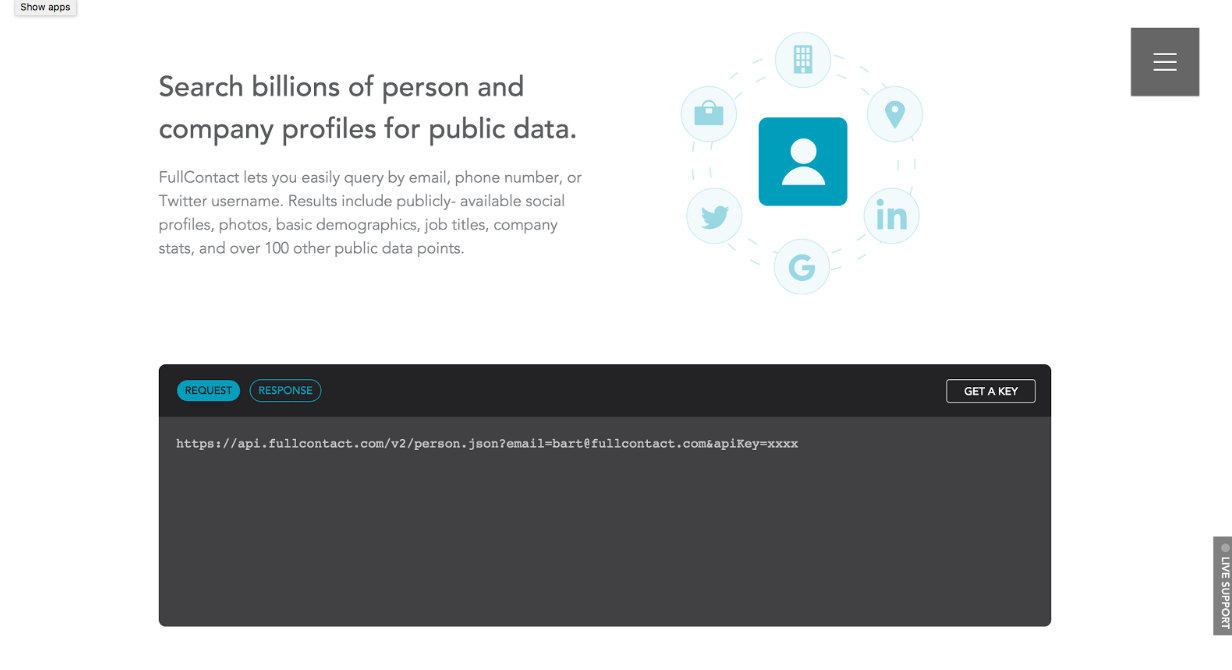
\includegraphics[scale=0.8]{fullContact.png}  
  \caption{FullContact}
	\label{fig:fc}
\end{figure}

Преимущества:
\begin{itemize}
\item предоставляет всевозможную публичную информацию об интересующих объектах;
\item простая интеграция;
\item оплата зависит от количества произведенных запросов.
\end{itemize}
Недостатки:
\begin{itemize}
\item является всего лишь сервисом по предоставлению публичной информации;
\item оплата зависит от количества произведенных запросов.
\end{itemize}

\pagebreak
\subsection{Постановка задачи}
\label{sub:alternatives:task}
Таким образом, проанализировав существующие готовые решения, было решено разработать программное средство предоставляющие возможность объединить их преимущества вместе и сынтегрировать их все в одну платформу. Оно должно обладать следующими свойствами:

\begin{itemize}
\item легко интегрироваться с другими программными средствами и горизонтально масштабироваться; 
\item иметь интеграцию с онлайн чатом CRM Salesforce;
\item иметь функционал трекинга событий произведенных пользователем на сайте;
\item иметь панель администратора, включающую в себя: просмотр статистики по пользователям как для выбранного периода времени, так и в режиме онлайн, возможность добавления администраторами и менеджерами новых событий в любое время;
\item интеграция с FullContacts для собирания публичной информации о пользователе из доступных социальных сетей, фотографий, географического положения, карьере и других различных данных о пользователе;
\item отказоустойчивость.
\end{itemize}
